\section{Methodology}\label{sec:methodology}
We collected subjective responses and physiological data from human subjects using wearable devices, personal data using surveys, and environmental data using data loggers.
We then applied supervised machine learning algorithms to train personal thermal comfort models for each study participant.
Thermal preference votes from the \ac{rhrn} survey (i.e., Q.1 Cozie Survey -- Thermal preference -- please see Section~\ref{subsec:surveys}) were utilized as the ground truth labels for model training and evaluation.
The methodology and sensors we used to measure and log data are summarized in Figure~\ref{fig:study_methodolgy}, while a flowchart depicting the methodology we used to analyze the data is shown in Figure~A.2.
The human subject experiment for this study was approved by the University of California Berkeley IRB (Institutional Review Board: 2020-01-12899).
We compensated participants who completed the study with gift vouchers for a total amount of SGD 400. 

\begin{figure}[thb!]
    \centering
    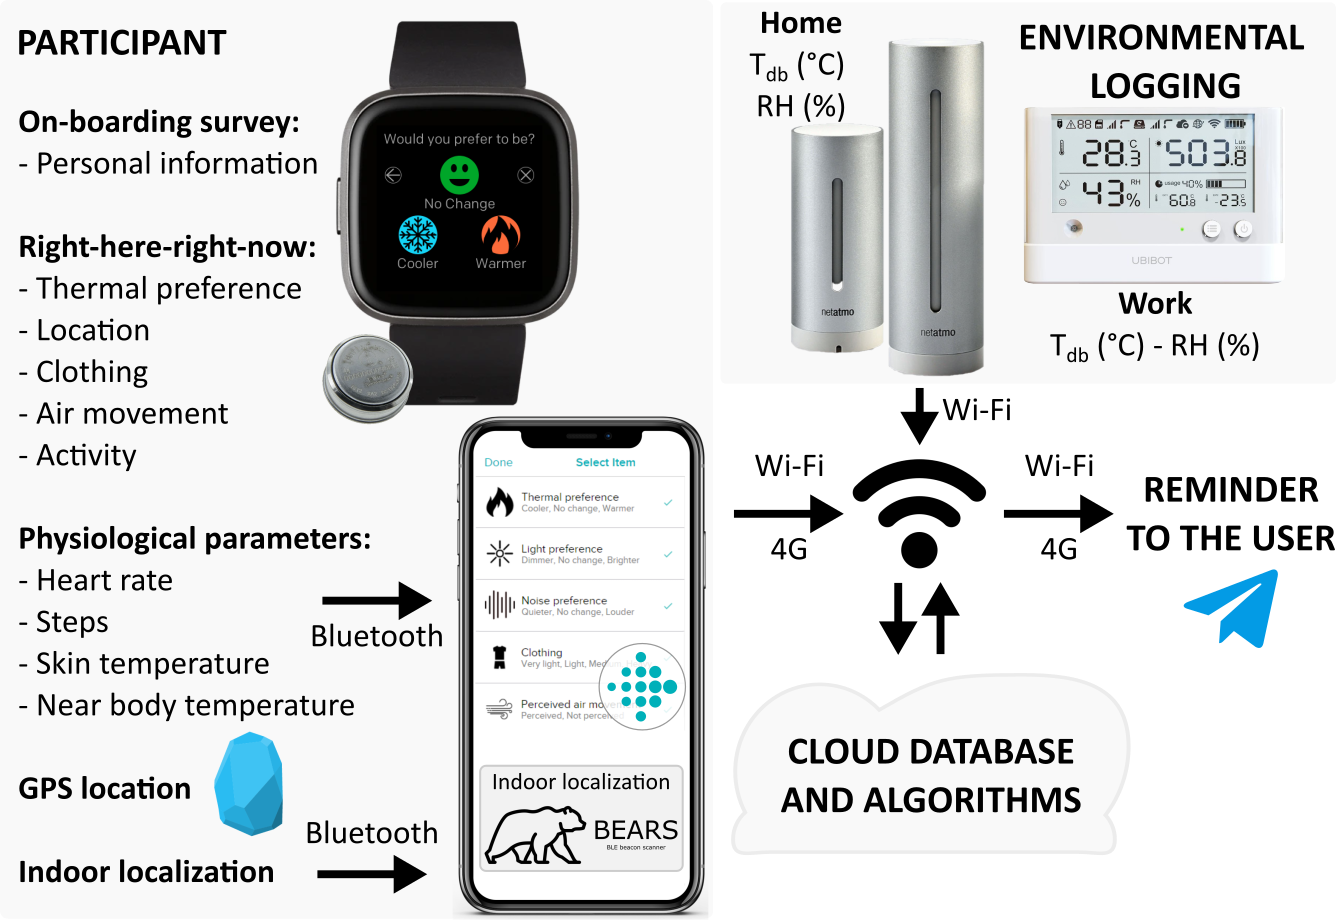
\includegraphics[width=\textwidth]{figures/figure_1}
    \caption{Methodology used to collect data in our study.
    Participants answered the \ac*{rhrn} surveys using the Fitbit Cozie clock-face.
    Physiological data and \ac*{rhrn} responses were first sent to the Fitbit companion application and then synced with a cloud database.
    The \ac*{hr} data were downloaded from the Fitbit accounts.
    \Ac*{t-sk-w} and \ac*{t-nb} were measured using two \glspl{ib} which were installed on the Fitbit wristband.
    Indoor location was monitored using two BLE beacons communicating with the BEARS Android application when each participant's phone was in their proximity.
    Environmental data were uploaded to the cloud database using Wi-Fi.
    Finally, participants were reminded to complete the \ac*{rhrn} surveys using Telegram, a messaging application.}
    \label{fig:study_methodolgy}
\end{figure}

\subsection{Subjects}\label{subsec:subjects}
Participants were recruited through online posting.
The inclusion criteria were that the participant must: have lived for at least three months in Singapore, be at least 21 years old, and be fluent in English.
Personal information (e.g., sex, age, education) about participants was collected using a web-based survey at the beginning of the study.

\subsection{Wearable sensors}\label{subsec:wearables}
Each participant received a Fitbit Versa (v1 or v2) and was asked to wear it daily for the whole duration of the study.

To measure and log \ac{t-sk-w} and \ac{t-nb} we installed two \glspl{ib}, model DS1925, on the Fitbit wristband.
One \gls{ib} was installed on the inner side of the wristband and measured \ac{t-sk-w} in the front part of the wrist.
The other was installed above the watch display and was used to measure \ac{t-nb}.
Figure~A.1 shows the exact location of where the \glspl{ib} were installed.

More information about the rationale on why we used Fitbit and \gls{ib} can be found in Section~1 of the Appendix.

Participants were asked to complete the \ac{rhrn} not sooner than 10 minutes after either wearing the Fitbit or changing clothes or activity.
This further limits the error in the measurement of \ac{t-sk-w} and ensured that they did not complete a \ac{rhrn} survey during a transitory.

\subsection{Environmental sensors}\label{subsec:environmental-loggers}
Environmental data was monitored and logged using three sensors.
One was installed in the room of their house, where they spent the majority of their time indoors.
This room corresponds to the `Home' location in question three of the Cozie survey as shown in Figure~\ref{fig:cozie_flow}.
Another was used to measure and log \ac{t-db} and relative humidity at the participant's workplace.
This room corresponds to the `Work' location in the Cozie survey.
The workstation could be in their office or home if they were working from home.
Finally, the third sensor on a bag/backpack of their choice.
Participants were instructed to select `Portable' in question three when within a 2~m radius of this sensor.
Detailed information about each sensor used are presented in Section~1 of the Appendix and Table~A.1.

\subsection{Surveys}\label{subsec:surveys}
Participants were asked to complete, on average, a total of 42 \ac{rhrn} surveys per week over a period of 180 days using the Cozie clock-face.
Figure~\ref{fig:cozie_flow} shows the flow of questions that were included in the \ac{rhrn} survey.

\begin{figure}[thb!]
    \centering
    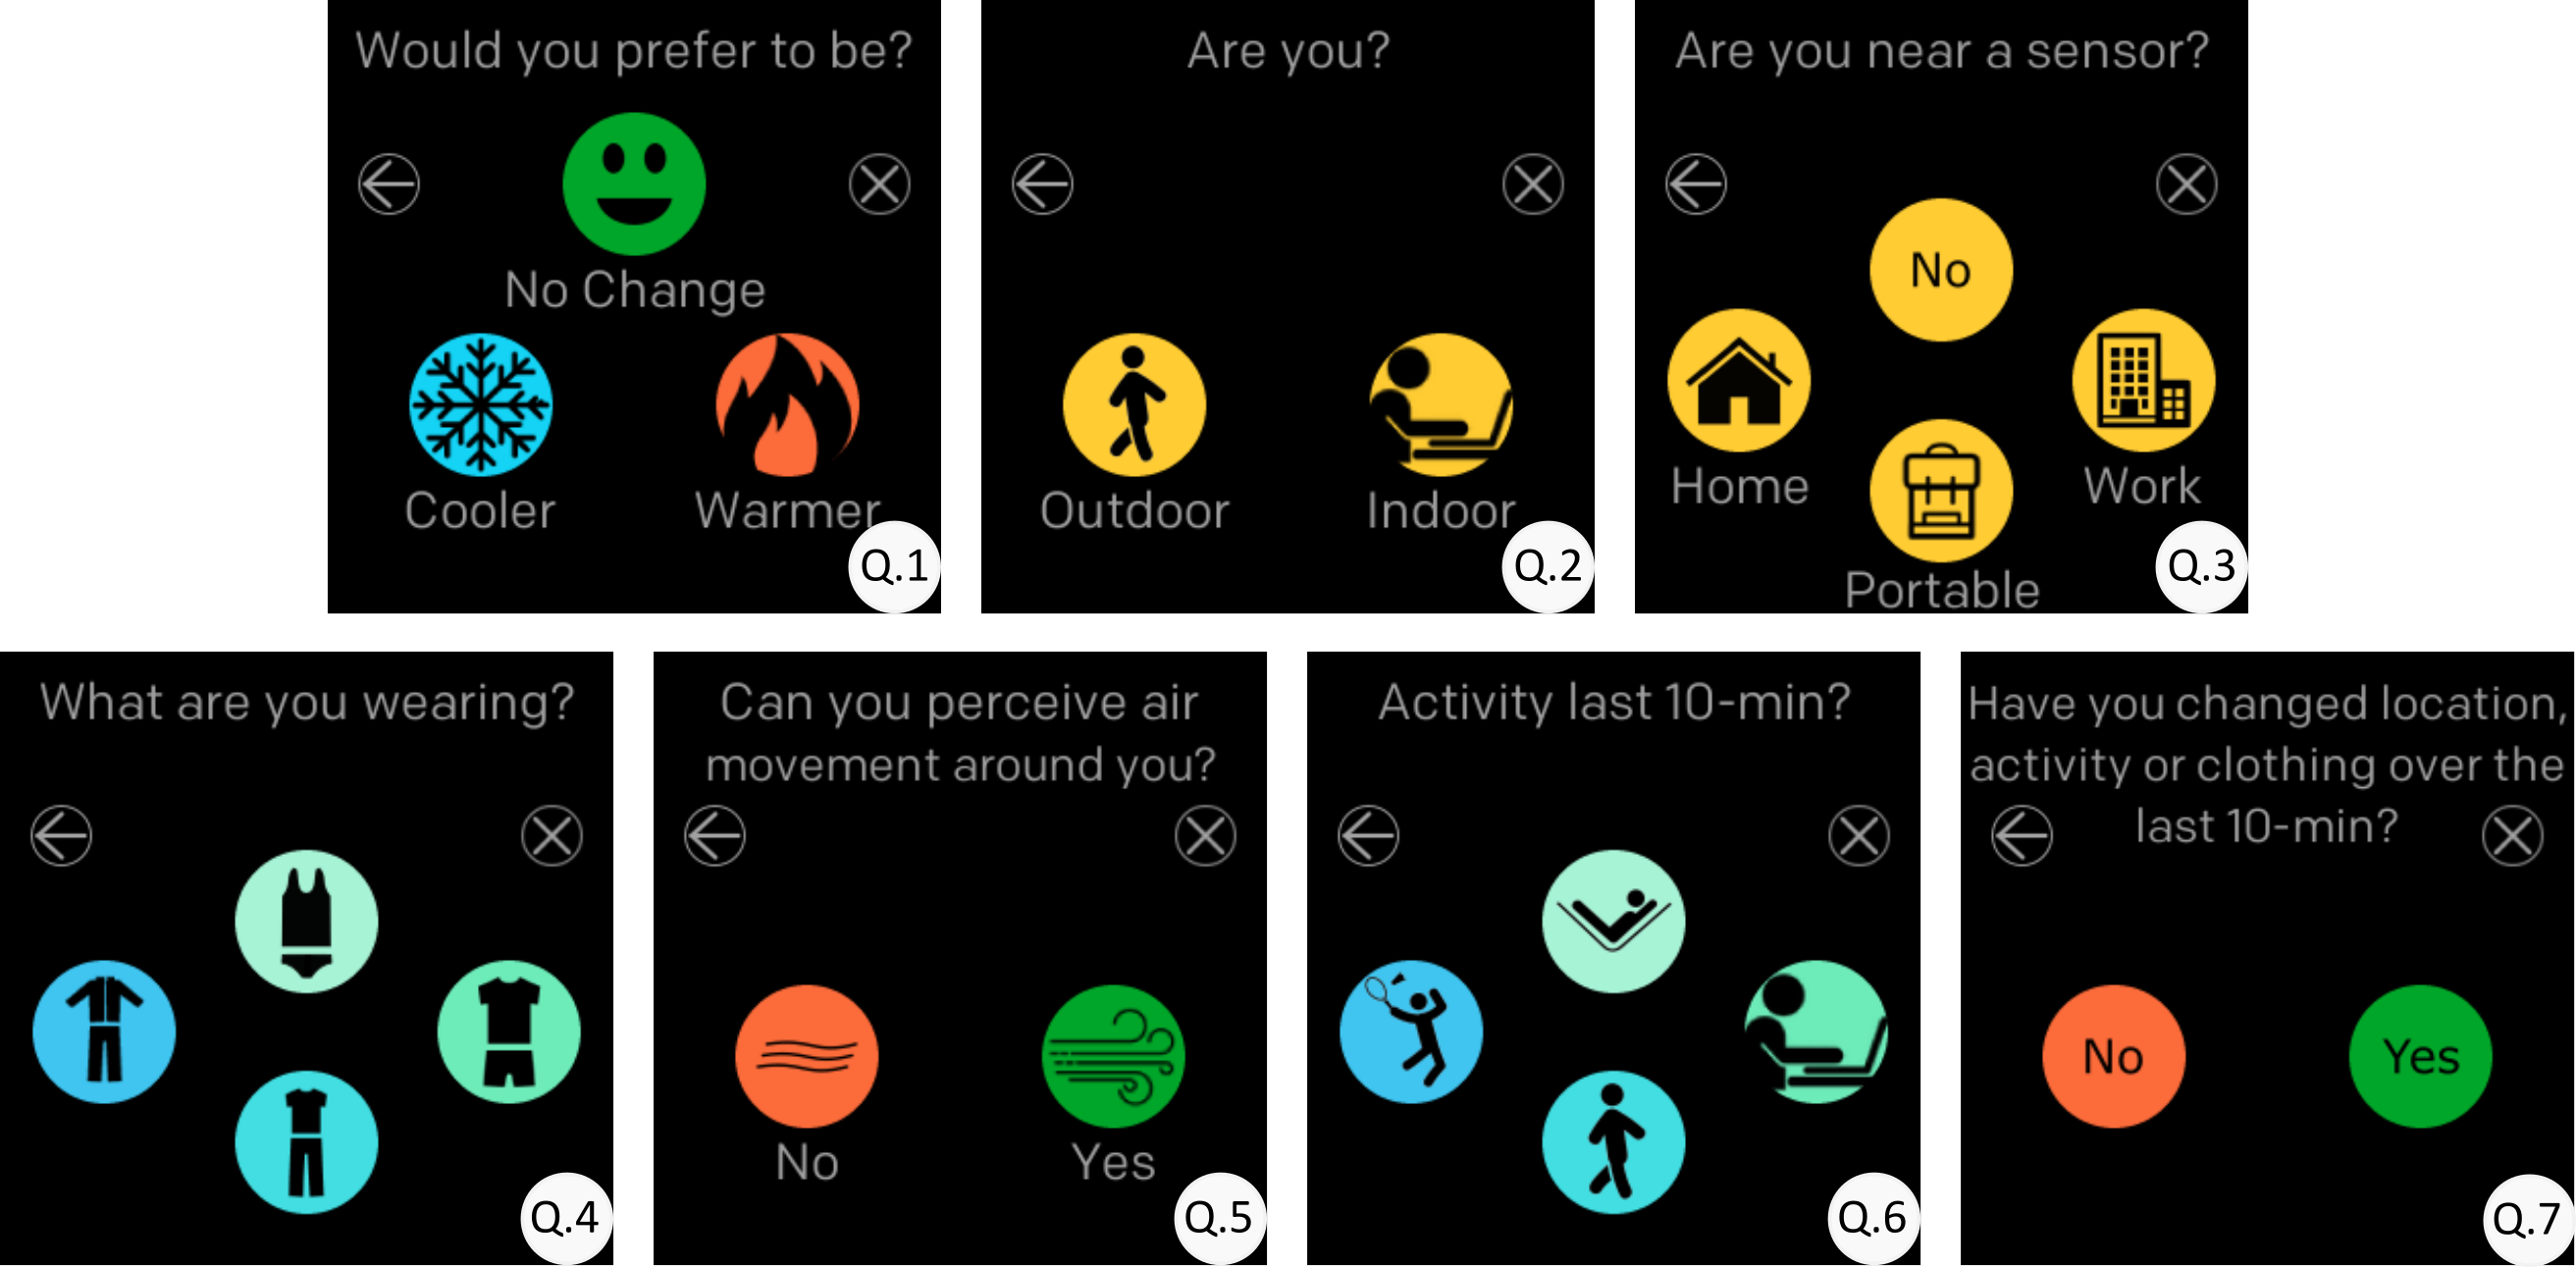
\includegraphics[width=\textwidth]{figures/figure_2}
    \caption{\acf{rhrn} survey questions displayed using the Cozie clock-face.}
    \label{fig:cozie_flow}
\end{figure}

Q.1 -- `Would you prefer to be?' assesses the thermal preference using a three-point scale.
Q.2 -- `Are you?' logs if participants completed the survey either indoors or outdoors.
Q.3 -- `Are you near a sensor?' determines if a participant is in proximity to one of the three environmental sensors.
Q.4 -- `What are you wearing?' participants reported their clothing level using a 4-point ordinal scale.
Q.5 -- `Can you perceive air movement around you?' assesses if the air surrounding the participant was still.
Q.6 -- `Activity last 10-min?' participants reported their activity level over the last 10 minutes.
Q.7 -- logged if the survey is answered during a transitory situation or in a near `steady-state' environment.

The questions flow was always displayed in the same order.
A custom-made algorithm analyzed real-time environmental data and occupants' indoor location that was logged by an application we developed.
Participants received a message when in the proximity of the two environmental sensors, and they had completed less than 10~\% of the total \ac{rhrn} surveys in those environmental conditions.

\subsection{Weather data}\label{subsec:weather-data}
Weather data were obtained from the Singapore Government website that provides 1-minute interval data~\cite{DataGovSGWeather}.
Weather data was merged with the GPS information collected by the Cozie app and answers to question two of the \ac{rhrn} survey.

\subsection{Data analysis}\label{subsec:data-analysis}
The source code we used to analyze the data and the full dataset are publicly available at this URL: \url{https://github.com/FedericoTartarini/dorn-longitudinal-tc-study}.

\subsubsection{Data preparation}\label{subsubsec:data-preparation}
Participants completed surveys while performing a wide range of activities, wearing different clothing, being in multiple locations, and being exposed to a broad range of environmental conditions.

We aimed to develop a personal thermal comfort model for each participant, which could potentially be used to better control and operate buildings.
Consequently, we decided to exclude the responses that participants provided:
(i) while exercising,
(ii) when not in the proximity of either of the environmental sensors provided (answered `No' to Q.3),
(iii) during a transitory situation (answered `Yes' to Q.7),
(iv) when outdoors,
(v) while not wearing the smartwatch correctly.
The rationale behind our decisions was that personal comfort models could mainly be used indoors to improve thermal comfort conditions where environmental conditions can be controlled.
We provide a detailed description of how we implemented the above-mentioned selection criteria in Section~2 of the Appendix.

\subsubsection{Supervised machine learning algorithms}\label{subsubsec:alogorithms}
We used seven supervised machine learning classifiers to predict thermal preferences: \gls{lr}, \gls{rdf}, Extreme Gradient Boosting, \ac{svm}, K-Nearest Neighbors, Gaussian Naive Bayes, and Multi-Layer Perceptron.
We used the Kruskal-Wallis H-test to test the null hypothesis that the population median of all the groups is equal.
The Kruskal-Wallis H-test was used since the ANOVA assumptions were not satisfied, and it is a non-parametric version of ANOVA.\@
The rejections of the null hypothesis do not indicate which of the groups differs. 
Comparisons between groups are required to determine which groups are different.

\subsubsection{Training data size}\label{subsubsec:pm}
One of our objectives was to determine how the number of training data points would affect the model accuracy.
This has practical applications since it would inform us of the minimum required number of \ac{rhrn} to be collected from each participant.
The hypothesis is that a higher number of data for each participant would lead to more accurate results.
To test this, we randomly selected 100 data points for testing and then trained the models using the first 42 \ac{rhrn} surveys (approximately one week of data) each participant completed.
We then iteratively trained a new model for each increment which comprised additional 84 training data points.

\subsubsection{Independent variable selection}\label{subsubsec:feature-selection}
The independent variables we used to train our models are shown in Table~\ref{tab:features}.
Each column represents a sub-set of variables and each row the respective model.
The variables were grouped as follows:
\textbf{\textit{environmental}} -- outdoor air temperature, outdoor humidity ratio, \acf{t-db}, and \acf{w-i};
\textbf{\textit{clo--met}} -- self-reported clothing and activity as explained in Section~\ref{subsec:surveys};\
\textbf{\textit{wearable}} -- location, \acf{hr}, \acf{t-sk-w}, and \acf{t-nb};\
\textbf{\textit{time}} -- hour of the day, weekday or weekend, and day of the week.
\begin{table}[h!]
    \centering
    \caption{Independent variables used to train the respective model. We used the following abbreviations in the table: self-reported clothing and activity (clo--met), environmental (env), wearable (wear), historical (hist).}
    \label{tab:features}
    \small \begin{tabular}{ccccccc}
               \toprule
               & \multicolumn{6}{c}{Variable sets} \\
               \cmidrule(lr){2-7}
               model              & \rotatebox{90}{env} & \rotatebox{90}{time} & \rotatebox{90}{wear} & \rotatebox{90}{clo--met}  & \rotatebox{90}{env-hist} & \rotatebox{90}{wear-hist} \\
               \midrule
               Thermal preference PCM  & x                   & x                    & x                    &                          &                         &                          \\
               Thermal preference PCM clo--met     & x                   & x                    & x                    & x                        &                         &                          \\
               Thermal preference PCM clo--met hist & x                   & x                    & x                    & x                        & x                       & x                        \\
               \bottomrule
    \end{tabular}
\end{table}


We also computed some variables (\textbf{\textit{hist}}) to take into account how thermal history may have influenced how participants perceived their environment at the time of completing the \ac{rhrn} survey.
For each of the time-series data included in either the \textit{environmental} or the \textit{wearable} variable sets, we calculated the following additional variables: exponentially weighted moving average and gradient over a 20 and 60 minutes period preceding the survey.
Average and gradient for the weather data were calculated using timeframes of 1 and 8 hours.

We used the \gls{shap} to determine how much each variable influences the output of the model.
The primary idea behind Shapley value-based explanations of machine learning models is to divide the credit for a model's output among its input variables using fair allocation outcomes from cooperative game theory~\cite{NIPS2017_7062, shap2016}.
The use of the \gls{shap} approach allowed us to understand and interpret how and why our complex models made
specific predictions.

We included \textit{env}, \textit{time}, and \textit{wearable} in all models since previous research has demonstrated that the inclusion of these variables into personal comfort models significantly increases their prediction accuracy~\cite{Liu2019a}.
We, therefore, decided only to test whether the use of historical and self-reported clothing and activity would have improved the prediction accuracy in our case.

We have shared the data we collected publicly so other researchers may test different hypotheses or use a different approach from the one described in this paper.

Including \acf{t-db}, \acf{t-sk-w}, and \acf{t-nb} to all models may introduce multicollinearity.
The environment to which a person is exposed, the clothing they wear, and the actions they perform, together which several other factors affect how \acf{t-db}, \acf{t-sk-w}, and \acf{t-nb} are correlated.
We, therefore, decided to keep them all in the models since they allowed us to potentially capture all the above-mentioned interactions that cannot be measured but still play a significant role in how people perceive their thermal environment.
For example, the near body temperature may approximate the air temperature when a person is exposed to elevated air speeds. On the other hand, it will be more influenced by the skin temperature when the person is resting and the air in the room is still. 
It is worth mentioning that Apple in their latest smartwatch, the Apple Watch 8 released in October 2022, also included two temperature sensors, one that measures the skin temperature and one below the screen to isolate the body temperature from the outside environment. 
Apple claims that this allows them to get a more accurate estimate of the variables that they want to predict~\cite{apple2022}.

\subsection{PMV estimation}\label{subsubsec:pmv-estimation}
We used the measured environmental variables and personal factors, qualitatively logged by the participants to calculate the \ac{pmv} using the following assumptions.
The activity levels reported by the participants were mapped using the following values resting~=~0.8~met, sitting~=~1.1~met, and standing~=~1.4~met.
While reported clothing values were mapped as follows very light~=~0.3~clo, light~=~0.5~clo, medium~=~0.7~clo, and heavy~=~1.0~clo.
These numbers were determined by asking each participant which clothes on average they wore when selecting one of the above options.
The mean radiant temperature was assumed to be equal to \ac{t-db}~\cite{Dawe2020}.
The relative airspeed value was calculated assuming the airspeed to be equal to 0.1~m/s and using the self-reported activity levels.
We are fully aware that these assumptions have limitations and do affect the \ac{pmv} prediction accuracy;\
however, similar assumptions have been previously used in thermal comfort research~\cite{Kim2018}.
Finally, we mapped the \ac{pmv} values into thermal preference votes using the following assumptions: `Warmer' for \ac{pmv} $<$ 1.5, `Cooler' for \ac{pmv} $>$ 1.5, and `No Change' for -1.5 $\leq$ \ac{pmv} $\leq$ 1.5.
This is the same assumption made by Fanger who considers dissatisfied those people who reported their absolute value of thermal sensation to be either 2 or 3~\cite{Fanger1970}.
This is based on the assumption that, for example, people who have a thermal sensation of `Warm' or `Hot' is highly probable that they may want to be `Cooler'.
In this paper, we did not draw conclusions on the accuracy of the \ac{pmv} model, but we only used it as a benchmark value to assess the accuracy of the thermal personal comfort models.

\subsubsection{Evaluation criteria}\label{subsubsec:evaluation-criteria}
The model prediction accuracy was evaluated using the following metrics: F1-micro, F1-macro, and Cohen's kappa.
We calculated all these metrics for a more precise interpretation of the results, however, we only reported the F1-micro scores unless there was a significant disagreement between the prediction accuracy scores of different metrics.
F1-micro ranges between 0 and 1 where 1 represents the optimal prediction value.
F1-micro measures the prediction accuracy and gives equal importance to precision (true positives divided by all positive results) and recall (true positives divided by the number of samples that should have been identified as positives).
In multilabel classification, (i.e., in our case since thermal preference assumes three values) the F1-micro is calculated globally across all classes.
We did not use nor report the simple accuracy metric (i.e., how many observations, both positive and negative, were correctly classified) since it should not be used for imbalanced problems.
In imbalanced scenarios, our dataset, high accuracy score can simply be obtained by classifying all observations as the majority class.

\subsubsection{Training and testing}\label{subsubsec:train-test}
Hyper-parameters optimization is done by using a random search and 5-fold cross-validation.
We tested ten random combinations of hyper-parameters in each of the 5-fold, and the best performing model, in terms of objective metric as specified in Section~\ref{subsubsec:evaluation-criteria}, is chosen.
Table~A.2 shows the parameters chosen for training the models and performing the random search.
We repeated this entire process 100 times for each model.